%%%%%%%%%%%%%%%%%%%%%%%%%%%%%%%%%%%%%%%%%
% Beamer Presentation
% LaTeX Template
% Version 1.0 (10/11/12)


\documentclass{beamer}

\mode<presentation> {

% The Beamer class comes with a number of default slide themes
% which change the colors and layouts of slides. Below this is a list
% of all the themes, uncomment each in turn to see what they look like.

%\usetheme{default}
%\usetheme{AnnArbor}
%\usetheme{Antibes}
%\usetheme{Bergen}
%\usetheme{Berkeley}
%\usetheme{Berlin}
%\usetheme{Boadilla}
%\usetheme{CambridgeUS}
%\usetheme{Copenhagen}
%\usetheme{Darmstadt}
%\usetheme{Dresden}
%\usetheme{Frankfurt}
%\usetheme{Goettingen}
%\usetheme{Hannover}
%\usetheme{Ilmenau}
%\usetheme{JuanLesPins}
%\usetheme{Luebeck}
\usetheme{Madrid}
%\usetheme{Malmoe}
%\usetheme{Marburg}
%\usetheme{Montpellier}
%\usetheme{PaloAlto}
%\usetheme{Pittsburgh}
%\usetheme{Rochester}
%\usetheme{Singapore}
%\usetheme{Szeged}
%\usetheme{Warsaw}

% As well as themes, the Beamer class has a number of color themes
% for any slide theme. Uncomment each of these in turn to see how it
% changes the colors of your current slide theme.

%\usecolortheme{albatross}
%\usecolortheme{beaver}
%\usecolortheme{beetle}
%\usecolortheme{crane}
%\usecolortheme{dolphin}
%\usecolortheme{dove}
%\usecolortheme{fly}
%\usecolortheme{lily}
%\usecolortheme{orchid}
%\usecolortheme{rose}
%\usecolortheme{seagull}
%\usecolortheme{seahorse}
\usecolortheme{whale}
%\usecolortheme{wolverine}

%\setbeamertemplate{footline} % To remove the footer line in all slides uncomment this line
%\setbeamertemplate{footline}[page number] % To replace the footer line in all slides with a simple slide count uncomment this line

%\setbeamertemplate{navigation symbols}{} % To remove the navigation symbols from the bottom of all slides uncomment this line
}

\usepackage{graphicx} % Allows including images
\usepackage{booktabs} % Allows the use of \toprule, \midrule and \bottomrule in tables
\usepackage{listings}
\usepackage{color}
\usepackage{multirow}
\usepackage{hhline}


\definecolor{dkgreen}{rgb}{0,0.6,0}
\definecolor{gray}{rgb}{0.5,0.5,0.5}
\definecolor{mauve}{rgb}{0.58,0,0.82}

\lstset{frame=tb,
  language=R,
  aboveskip=1mm,
  belowskip=1mm,
  showstringspaces=false,
  columns=flexible,
  basicstyle={\tiny  \ttfamily},
  numbers=none,
  numberstyle=\tiny\color{gray},
  keywordstyle=\color{blue},
  commentstyle=\color{dkgreen},
  stringstyle=\color{mauve},
  breaklines=true,
  breakatwhitespace=true,
  tabsize=3
}

%----------------------------------------------------------------------------------------
%	TITLE PAGE
%----------------------------------------------------------------------------------------

\title[Graph Search]{Graph Search} % The short title appears at the bottom of every slide, the full title is only on the title page

%\author{} % Your name
\institute[Parallel Programming] % Your institution as it will appear on the bottom of every slide, may be shorthand to save space
{
\large{Parallel Programming} \\
\large{} % Your institution for the title page
\medskip
%\textit{john@smith.com} % Your email address
}
\date{\today} % Date, can be changed to a custom date

%%%%%%%%%%%%%%%%%%%%%%%%%%%%%%%% Document Started %%%%%%%%%%%%%%%%%%%%%%%%%

\begin{document}

%%%%%%%%%%%%%%%%%%% Title Page %%%%%%%%%%%%%%%%%%%%%%%%%%%%%%%%%%%
\begin{frame}
\titlepage % Print the title page as the first slide
\end{frame}

%%%%%%%%%%%%%%%%%%%%%%%%%%%%%%% Title Page Over %%%%%%%%%%%%%%%%%%%%%%%%%%%%




%%%%%%%%%%%%%%%%%%%%%%%%%%%%%% Slide-1  %%%%%%%%%%%%%%%%%%%%%%%%%%%%%%%%%%%
\begin{frame}
\frametitle{Graphs}
A graph is a finite set of nodes with edges between nodes.\\
Formally, a graph G is a structure (V,E) consisting of\\ 
\begin{itemize}
\item a finite set V called the set of nodes, and
\item a set E that is a subset of VxV. That is, E is a set of pairs of the form (x,y) where x and y are nodes in V 

\end{itemize}
\end{frame}



%%%%%%%%%%%%%%%%%%%%%%%%%%%%%%%%% Slide-2 %%%%%%%%%%%%%%%%%%%%%%%
\begin{frame}
\frametitle{Adjacency Matrix Representation}
%These are the incidents that happened at the Mexico  
\begin{itemize}
\item In this representation, each graph of n nodes is represented by an n x n matrix A, that is, a two-dimensional array A
\item The nodes are (re)-labeled 1,2,…,n
\item A[i][j] = 1 if (i,j) is an edge
\item A[i][j] = 0 if (i,j) is not an edge
\end{itemize}
\end{frame}
%%%%%%%%%%%%%%%%%%%%%%%%%%%%%%%%%%%%%%%%%
\begin{frame}
\frametitle{Example of Adjacency Matrix Representation}
%These are the incidents that happened at the Mexico

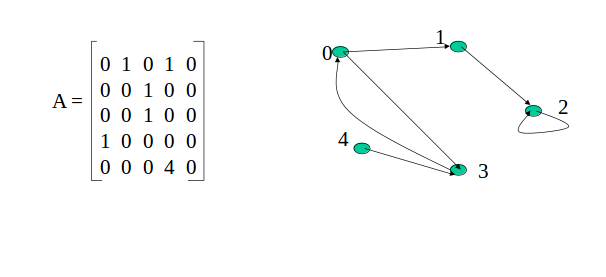
\includegraphics[width = 12cm]{mat2}
\end{frame}
%%%%%%%%%%%%%%%%%%%%%%%%%%%%%%%%% Slide-3 %%%%%%%%%%%%%%%%%%%%%%%
\begin{frame}
\frametitle{Graph Traversal}
Graph traversal (also known as graph search) refers to the process of visiting (checking and/or updating) each vertex in a graph. Such traversals are classified by the order in which the vertices are visited.\\
\begin{itemize}
\item There are two standard graph traversal techniques:\\
\begin{enumerate}
\item Depth-First Search (DFS)
\item Breadth-First Search (BFS)
\end{enumerate}
\end{itemize}
%%%%%%%%%%% Pending %%%%%%%%%%%%%%%%%%%%%%%%%%%%%%%%
\end{frame}


%%%%%%%%%%%%%%%%%%%%%%%%%%%%%%%%% Slide-4 %%%%%%%%%%%%%%%%%%%%%%%
\begin{frame}
\frametitle{Depth-First Search }
\begin{itemize}
\item DFS follows the following rules: 
\begin{enumerate}
\item Select an unvisited node x, visit it, and treat as the current node 
\item Find an unvisited neighbor of the current node, visit it, and make it the new current node; 
\item If the current node has no unvisited neighbors, backtrack to the its parent, and make that parent the new current node; 
\item Repeat steps 3 and 4 until no more nodes can be visited. 
\item If there are still unvisited nodes, repeat from step 1.
\end{enumerate}
\end{itemize}
\end{frame}


%%%%%%%%%%%%%%%%%%%%%%%%%%%%%%%%% Slide-5 %%%%%%%%%%%%%%%%%%%%%%%
\begin{frame}
\frametitle{Illustration of DFS}
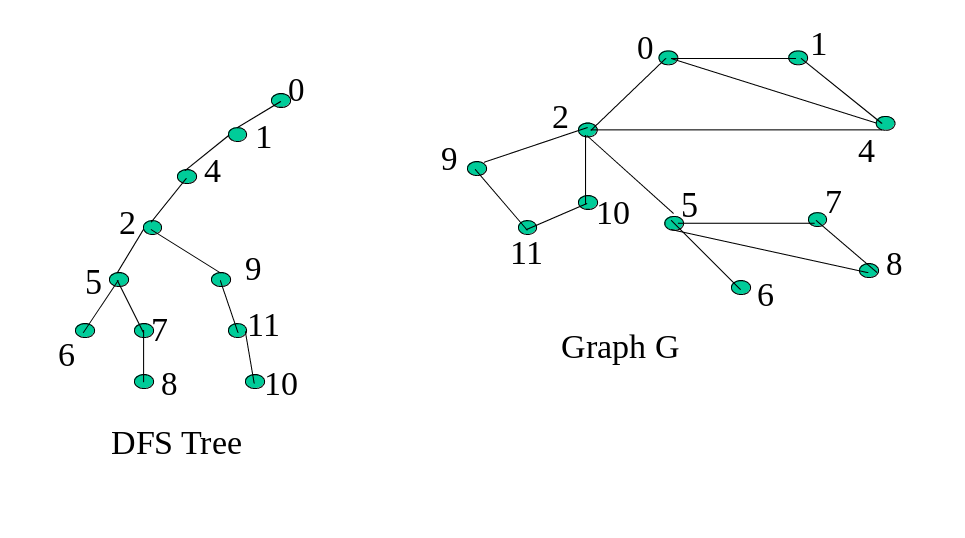
\includegraphics[height = 8cm,width = 12cm]{dfs}

\end{frame}


%%%%%%%%%%%%%%%%%%%%%%%%%%%%%%%%% Slide-6 %%%%%%%%%%%%%%%%%%%%%%%
\begin{frame}
\frametitle{DFS Algorithm}
Depth First Search algorithm(DFS) traverses a graph in a depthward motion and uses a stack to remember to get the next vertex to start a search when a dead end occurs in any iteration.\\
It employs following rules.
\begin{enumerate}
\item     Rule 1 - Visit adjacent unvisited vertex. Mark it visited. Display it. Push it in a stack.

\item    Rule 2 - If no adjacent vertex found, pop up a vertex from stack. (It will pop up all the vertices from the stack which do not have adjacent vertices.)

\item    Rule 3 - Repeat Rule 1 and Rule 2 until stack is empty.
\end{enumerate}
\end{frame}



%%%%%%%%%%%%%%%%%%%%%%%%%%%%%%%%% Slide-7 %%%%%%%%%%%%%%%%%%%%%%%
\begin{frame}[fragile]
\frametitle{Pseudo-Code}

\begin{lstlisting}

DFS(s,n)
{
push(s);
vis[s]=1 //set it as visited
k=pop();
if(k not equal to 0)
print k;
while(k not equal to 0)
{
for(i=1 to n)
if(a[k][i]not equal to 0 and node is not visited)
{
push(i);
vis[i]=1;// set it as visited
}
k=pop();
if(k not equal to 0)
print k;
}
for(i=1 to n)
if(node is not visited)
dfs(i,n);
}

\end{lstlisting}

\end{frame}


%%%%%%%%%%%%%%%%%%%%%%%%%%%%%%% Last Slide %%%%%%%%%%%%%%%%%%%%%%%%%%%%%
\begin{frame}
\frametitle{Breadth-First Search}
\begin{itemize}
\item BFS follows the following rules: 
\begin{enumerate}
\item Select an unvisited node x, visit it, have it be the root in a BFS tree being formed. Its level is called the current level. 
\item From each node z in the current level, in the order in which the level nodes were visited, visit all the unvisited neighbors of z. The newly visited nodes from this level form a new level that becomes the next current level. 
\item Repeat step 2 until no more nodes can be visited. 
\item If there are still unvisited nodes, repeat from Step 1.
\end{enumerate}
\end{itemize}

\end{frame}

\begin{frame}
\frametitle{Illustration of BFS}
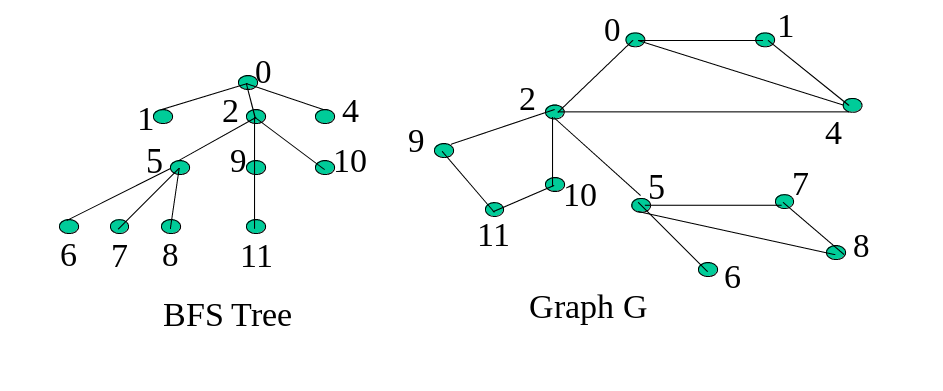
\includegraphics[width = 12cm]{bfs}
\end{frame}

\begin{frame}
\frametitle{BFS Algorithm}
Breadth First Search algorithm(BFS) traverses a graph in a breadthwards motion and uses a queue to remember to get the next vertex to start a search when a dead end occurs in any iteration. \\It employs following rules.
\begin{enumerate}

\item     Rule 1 − Visit adjacent unvisited vertex. Mark it visited. Display it. Insert it in a queue.

\item    Rule 2 − If no adjacent vertex found, remove the first vertex from queue.

\item     Rule 3 − Repeat Rule 1 and Rule 2 until queue is empty.
\end{enumerate}
\end{frame}

\begin{frame}[fragile]
\frametitle{Pseudo-Code}
\begin{lstlisting}

BFS(s,n)
{
Set all nodes to "not visited";
q.enqueue(initial node);
vis[s]=1//set it as visited
p=q.dequeue();
if(p is not zero)
print p;
while(p is not zero)
{
for(i=1 to n)
if(a[p][i] is not equal to 0 and node is not visited)
{
q.enqueue(i) //node i
vis[i]=1 //set it as visited
}
p=q.dequeue();
if(p is not equal to 0)
print p;
}
for(i=1 to n)
if (i is not visited)
BFS(i,n)
}

\end{lstlisting}
\end{frame}
\begin{frame}
\frametitle{Complexity}
\begin{table}[h!]
\begin{center}
\begin{tabular}{|c|c|c|}
\hline
Algorithm & Time & Space\\
\hline
BFS & O($|$V$|+|E|$)&O($|$V$|$) \\
\hline
DFS & O($|$V$|+|E|$)&O($|$V$|$) \\
\hline
\end{tabular}
\caption{Time and Space Complexity}
\end{center}
\end{table}

\end{frame}

\begin{frame}
\frametitle{Analysis : Scalability}
\textbf{Application Scalability} : Scalability is the capability of the system to handle a growing amount of work, or its potential to be enlarged in order to accommodate that growth.\\

\begin{table}[h!]
\begin{center}
\begin{tabular}{|c|c|c|c|}

\hline
%\hhline{~--}

    \multirow{2}{*}{Vertices} & \multicolumn{3}{c|}{Execution time}\\
[0.5ex]
    \hhline{~---} 
    & bfs &  dfs&total
 \\
 \hline
10&	0.000011&	0.00001&	0.000021\\
\hline
20&	0.000021&	0.000019&	0.00004\\
\hline
30&	0.000033&	0.000032&	0.000065\\
\hline
40&	0.000035&	0.000033&	0.000068\\
\hline
100&	0.000248&	0.000242&	0.00049\\
\hline
500&	0.002436&	0.002379&	0.004815\\
\hline
1000&	0.009886&	0.009677&	0.019563\\
\hline    

    \end{tabular}
\caption{Execution time for different graph size}

\end{center}
\end{table}

\end{frame}
\begin{frame}
\frametitle{Analysis : Scalability}
\begin{figure}[h!]
\center
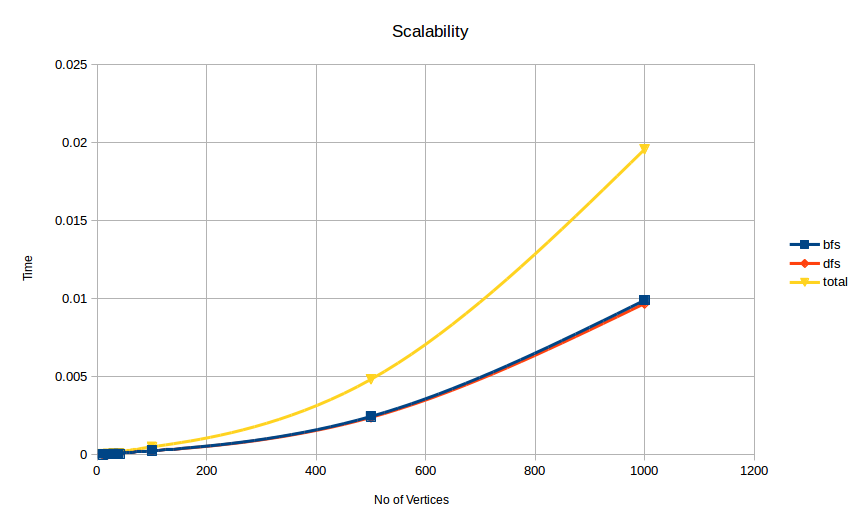
\includegraphics[width = 10cm]{image}
\caption{No. of Vertices Vs Time}
\end{figure}


\end{frame}
\begin{frame}
\frametitle{Analysis : CPU and Memory Requirement}\textbf{CPU and Memory requirement} : 

\begin{figure}[h!]
\center
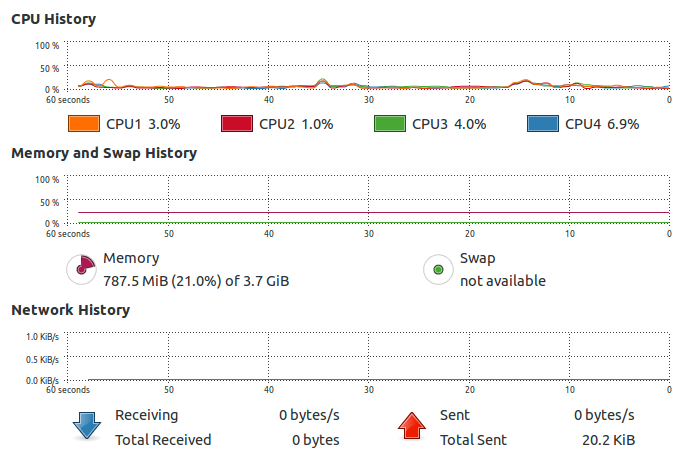
\includegraphics[width = 9cm]{gnome1}
\caption{gnome-system-monitor}
\end{figure}

\end{frame}

\begin{frame}
\frametitle{Analysis : Cache Misses}
\begin{figure}
\begin{center}
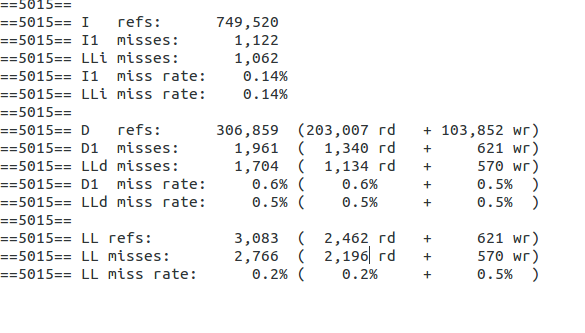
\includegraphics[width = 10cm]{misses}
\caption{Cache Misses}
\end{center}
\end{figure}
\end{frame}
\begin{frame}
\frametitle{Analysis : Cache Misses}
\begin{table}[h!]
\begin{center}
\begin{tabular}{|c|c|c|c|c|c|c|}

\hline
%\hhline{~--}

    \multirow{2}{*}{Vertices} & \multicolumn{3}{c|}{D1} &\multicolumn{3}{c|}{LL} \\
[0.5ex]
    \hhline{~------} 
&	Accesses	&\multicolumn{2}{c|}{Misses}	&Accesses	&\multicolumn{2}{c|}{Misses}\\
\hhline{~~--~--}
& & Read & Write & & Read & Write\\
\hline						
10&	82972&	1300&	546&	2968&	2171&	496\\
\hline
20	&168341	&1314	&568	&3004	&2180	&518\\
\hline
30	&306859	&1340	&621	&3083	&2196	&570\\
\hline
40	&498414	&1386	&698	&3206	&2218	&643\\
\hline
100	&2760300	&2559	&1308	&4993	&2231	&1198\\
\hline
500	&66608575	&33636	&16750	&51509	&2228	&16582\\
\hline
1000	&265688490	&129721	&64925	&195773	&62137	&64734\\
\hline

\end{tabular}
\caption{Cache Misses for different graph size}
\end{center}
\end{table}
\end{frame}
\begin{frame}\frametitle{Analysis : Cache Misses}
\begin{figure}
\begin{center}
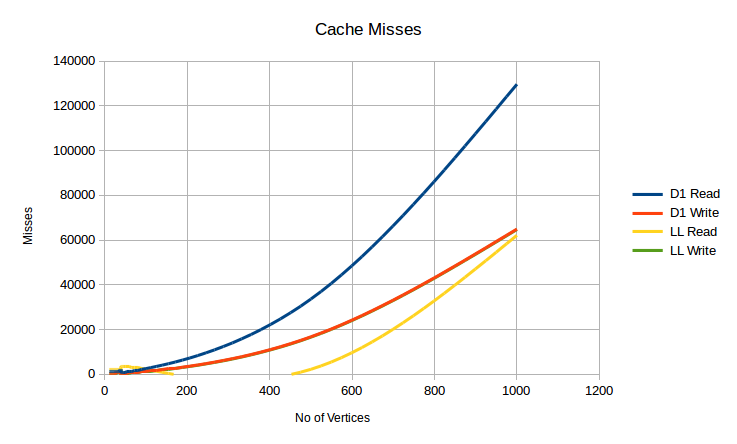
\includegraphics[width = 11cm]{cachemiss}
\caption{Cache Misses}
\end{center}
\end{figure}
\end{frame}

\begin{frame}
\frametitle{Analysis : Memory Leaks}
\begin{figure}
\begin{center}
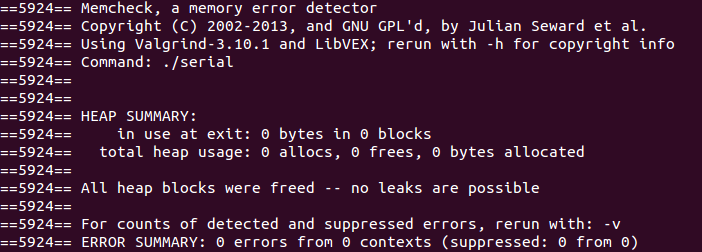
\includegraphics[width = 10cm]{memcheck}
\caption{Memory Leaks}
\end{center}
\end{figure}
\end{frame}

\begin{frame}
\frametitle{Analysis : Function Costs}
\begin{figure}
\begin{center}
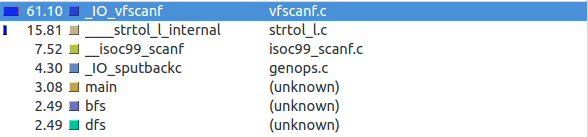
\includegraphics[width = 12cm]{kc1}\\
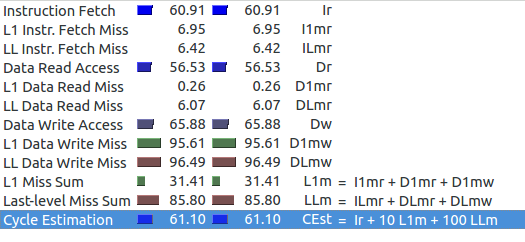
\includegraphics[width = 11cm]{kc2}

\caption{Analysis}
\end{center}
\end{figure}
\end{frame}

%\begin{frame}
%\frametitle{Future Work}
%identify Problematic areas which will be solved by parallel. 
%\end{frame}

\begin{frame}
\frametitle{}
\begin{center}
\large{Thank You}
\end{center}
\end{frame}


\begin{frame}
\frametitle{Team Members}
\center
\textbf{Rounak Jangir (201352028)}\\
\textbf{Anjul Tyagi (201351033)}\\
\textbf{Yash Choubey (201351006)}

\end{frame}

\end{document} 